\section{Automação}

\subsection{Infraestrutura como Código}

\subsection{Chef}
\label{sec:chef}

Chef é uma ferramenta de gerenciamento e configuração de infraestrutura criada
pela comunidade Opscode em 2008 oficialmente lançada em 2009. Seu propósito é
auxiliar na transformação de uma complexa infraestrutura em código, com nível
de abstração compreensiveis para os desenvolvedores. Sendo assim,
a gerência de configuração gira em torno da codificação simplificada e amigável
ao invés de comandos manuais de instalação e configuração de aplicações
\cite{sharma:2015}.

\begin{figure}[h]
  \label{fig:arch_chef}
  \centering
  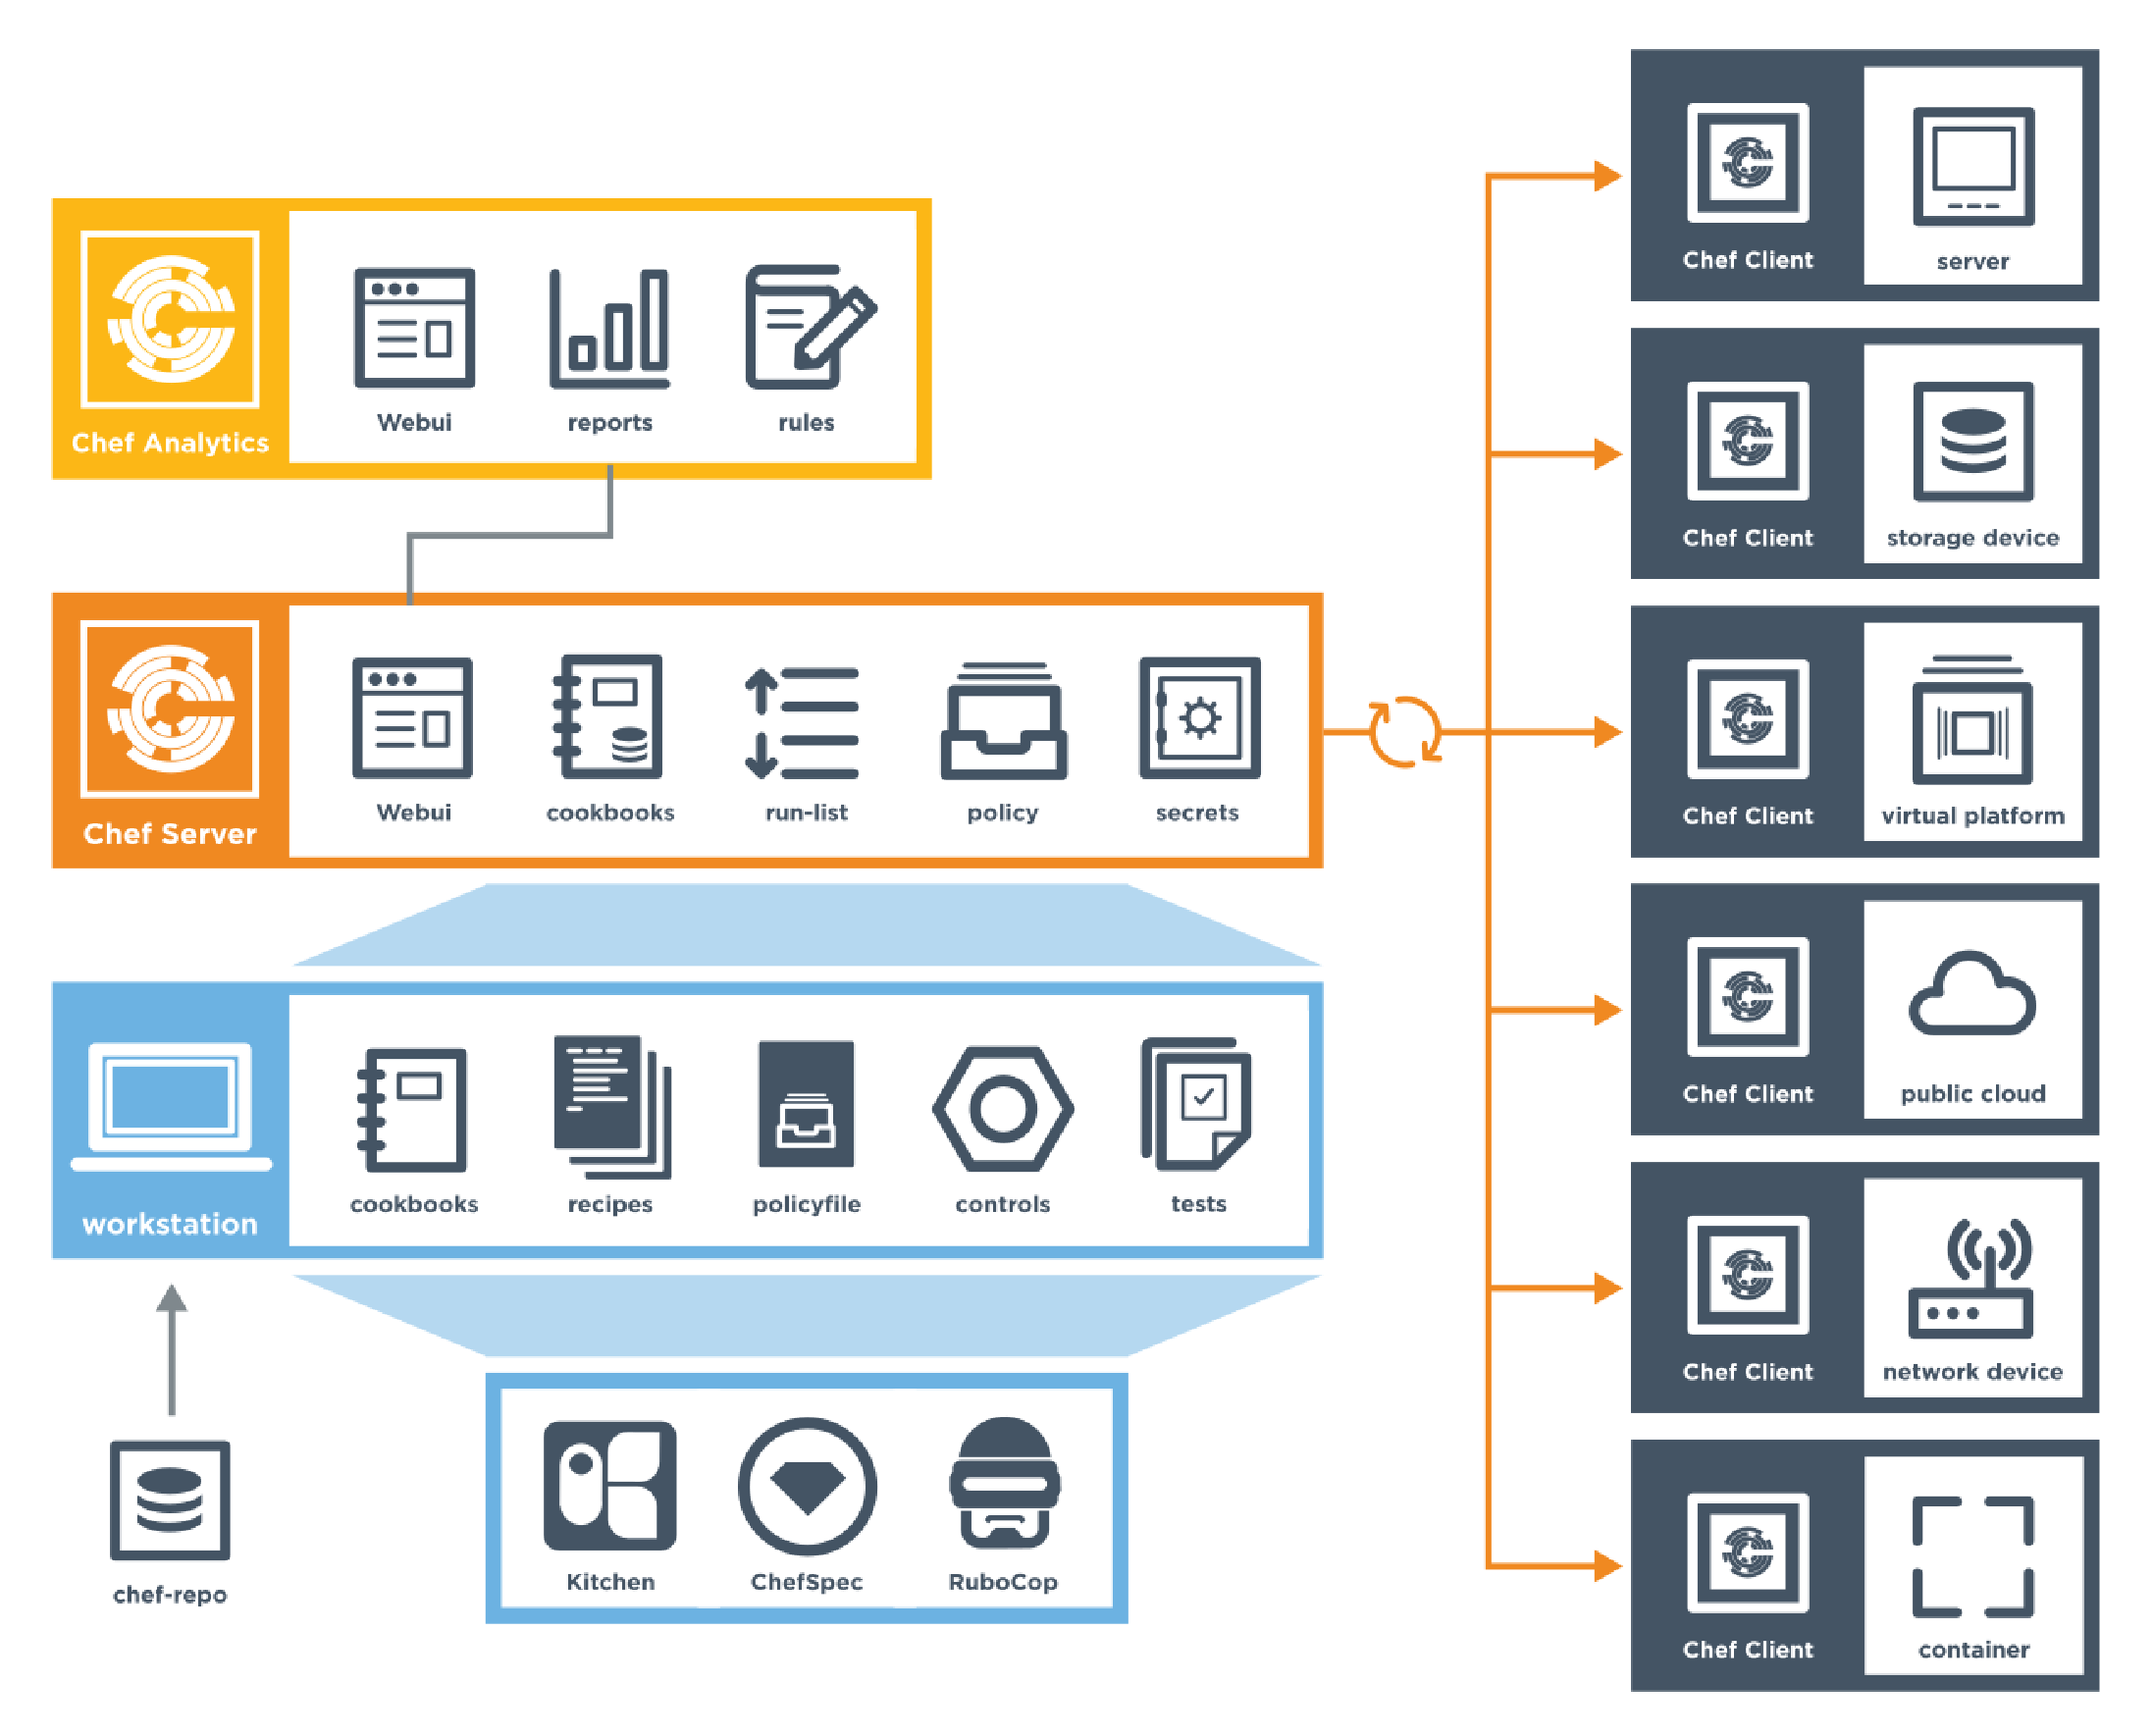
\includegraphics[width=\textwidth]{figuras/arch_chef.eps}
  \caption{Chef - Arquitetura de Componentes}
\end{figure}


